\def\fooA
{
    \begin{tikzpicture}
        \path[decorate,
            decoration={text along path,
                    text={Circumference},
                    text align=center}] (0,0) circle (-3.3 cm);
        \draw[ultra thick, black!60!green, ->] (0,0) -- (0,3);
        \draw (0.2,1.5) node[rotate=90, black!60!green] {Radius};
        \draw[thick] (0,0) circle (3);
        \draw[ultra thick, blue, <->] (-2.6,-1.5) -- (2.6,1.5);
        \draw[thick, fill=red, red] (0,0) circle (0.5mm) node[below, blue, rotate = 30] {Diameter};
    \end{tikzpicture}
}

\def\figRod
{
    \begin{figure}[H]
        \centering
        {
            \begin{tikzpicture}
                \draw (-3,1) -- (3,1);
                \draw (-3,-1) -- (3,-1);
                \draw (3,0) ellipse (0.2 and 1);
                \draw (-3,-1) arc (270:90:0.2 and 1);
                \draw[|->] (0,0) node[below] {$_o$} -- (1,0) node[right] {$x$};
                \draw[|-|] (-3,-1.5) -- (0,-1.5) node[below] {$2L$} -- (3,-1.5);
            \end{tikzpicture}
        }
        \caption{1D rod model for visualization (the length is only relevant in the $x$-dimension, all other dimensions should be assumed as zero) }
        \label{fig:Rod}
    \end{figure}
}

\def\figDescretizedDomain
{
    \begin{figure}[H]
        \centering
        {
            \begin{tikzpicture}
                % \draw[step=0.5cm, gray, very thin] (0,0) node[black, above=5mm] {$-L/2$} grid (8,0.5) node[black, above] {$+L/2$};
                \draw[step=0.5cm, gray, very thin] (0,0) grid (3.2,0.5);
                \draw[step=0.5cm, gray, very thin] (4.8,0) grid (8,0.5);
                \draw[|<->|] (0,-0.5) -- (8,-0.5);
                \draw[|-|] (1,0.7) -- (1.5,0.7);
                \draw[|->] (4,-0.15) node[below] {$_o$} -- (4.5,-0.15) node[right] {$x$};
                \node at (1.25,0.7) [above] {$h$};
                \node at (0,-0.5) [left] {$-L$};
                \node at (8,-0.5) [right] {$+L$};
                \node at (4,-0.5) [below] {$2L$};
                \foreach \x in {3.5,4,4.5} {
                        \foreach \y in {0.25} {
                                \fill[black] (\x, \y) circle (0.5mm);
                            }
                    }
            \end{tikzpicture}
        }
        \caption{Discretized domain of the 1D geometry from \autoref{fig:Rod}.}
        \label{fig:DescretizedDomain}
    \end{figure}
}

\def\figSolutionMat
{
    \begin{figure}[H]
        \centering
        {
            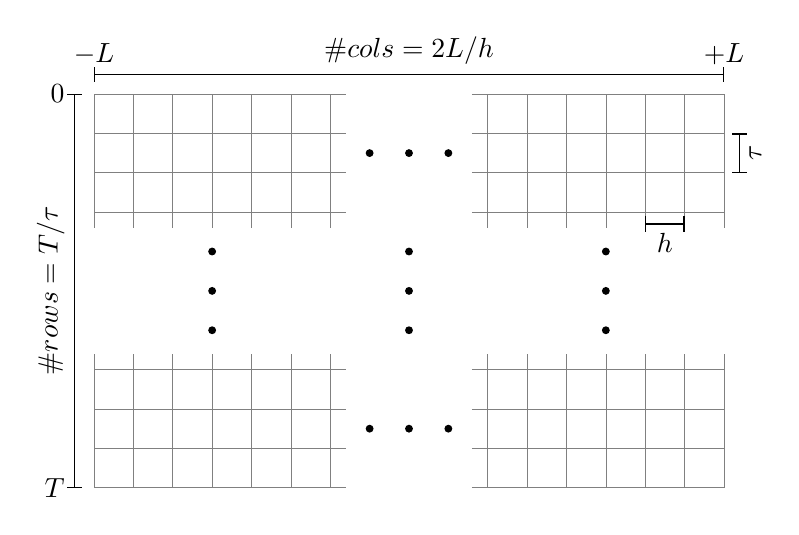
\begin{tikzpicture}
                % \draw[step=0.5cm, gray, very thin] (0,0) node[black, above=5mm] {$-L/2$} grid (8,0.5) node[black, above] {$+L/2$};
                \draw[step=0.5cm, gray, very thin] (0,0) grid (3.2,1.7);
                \draw[step=0.5cm, gray, very thin] (4.8,0) grid (8,1.7);
                \draw[step=0.5cm, gray, very thin] (0,3.3) grid (3.2,5);
                \draw[step=0.5cm, gray, very thin] (4.8,3.3) grid (8,5);
                \foreach \x in {3.5,4,4.5} {
                        \foreach \y in {0.75} {
                                \fill[black] (\x, \y) circle (0.5mm);
                            }
                    }
                \foreach \x in {1.5} {
                        \foreach \y in {2,2.5,3} {
                                \fill[black] (\x, \y) circle (0.5mm);
                            }
                    }

                \foreach \x in {4} {
                        \foreach \y in {2,2.5,3} {
                                \fill[black] (\x, \y) circle (0.5mm);
                            }
                    }

                \foreach \x in {6.5} {
                        \foreach \y in {2,2.5,3} {
                                \fill[black] (\x, \y) circle (0.5mm);
                            }
                    }

                \foreach \x in {3.5,4,4.5} {
                        \foreach \y in {4.25} {
                                \fill[black] (\x, \y) circle (0.5mm);
                            }
                    }


                \node at (4,5.25) [above] {$\text{\#cols}=2L/h$};
                \draw[|-|] (0,5.25) node[above] {$-L$} -- (8,5.25) node[above] {$+L$};

                \node at (-0.25,2.5) [above,rotate=90] {$\text{\#rows}=T/\tau$};
                \draw[|-|] (-0.25,0) node[left] {$T$} -- (-0.25,5) node[left] {$0$};

                \draw[|-|] (7,3.35) -- (7.5,3.35);
                \node at (7.25,3.35) [below] {$h$};

                \draw[|-|] (8.2,4) -- (8.2,4.5);
                \node at (8.2,4.25) [below,rotate=90] {$\tau$};

            \end{tikzpicture}
        }
        \caption{Solution Matrix. Each cell represents the value of $v$ at a particular time $\tau$ and space $h$. The boundaries are not shown as they are not part of the final solution.}
        \label{fig:SolutionMat}
    \end{figure}
}

\def\figDDecompose
{
    \begin{figure}[H]
        \centering
        {
            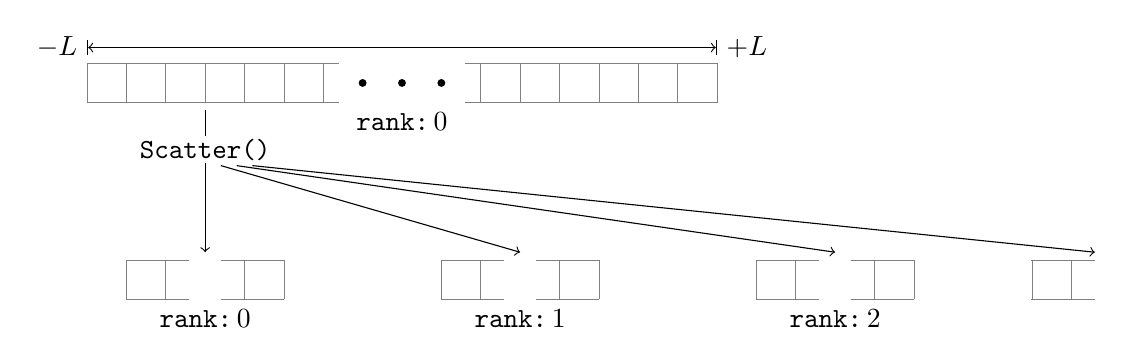
\begin{tikzpicture}
                % \draw[step=0.5cm, gray, very thin] (0,0) node[black, above=5mm] {$-L/2$} grid (8,0.5) node[black, above] {$+L/2$};
                \draw[|<->|] (-1.5,0.7) node[left] {$-L$} -- (6.5,0.7) node[right] {$+L$};
                \draw[step=0.5cm, gray, very thin] (-1.5,0) grid (1.7,0.5);
                \draw[step=0.5cm, gray, very thin] (3.3,0) grid (6.5,0.5);
                \foreach \x in {2,2.5,3} {
                        \foreach \y in {0.25} {
                                \fill[black] (\x, \y) circle (0.5mm);
                            }
                    }
                \node at (2.5,0) [below] {$\texttt{rank:}\, 0$};
                \begin{scope}[yshift=0]
                    \draw[->] (0,-0.1) -- (0,-0.6) node[fill=white, inner sep=1pt] {\texttt{Scatter()}} -- (0,-1.9);
                    \draw[->] (0.2,-0.8) -- (4,-1.9);
                    \draw[->] (0.4,-0.8) -- (8,-1.9);
                    \draw[->] (0.6,-0.8) -- (11.3,-1.9);

                    % \draw[step=0.5cm, gray, very thin] (-3.3,-2) grid (-2.5,-2.5);

                    \draw[step=0.5cm, gray, very thin] (-1,-2) grid (-0.2,-2.5);
                    \draw[step=0.5cm, gray, very thin] (0.2,-2) grid (1,-2.5);
                    \node at (0,-2.5) [below] {$\texttt{rank:}\, 0$};

                    \draw[step=0.5cm, gray, very thin] (2.99,-2) grid (3.8,-2.5);
                    \draw[step=0.5cm, gray, very thin] (4.2,-2) grid (5,-2.5);
                    \node at (4,-2.5) [below] {$\texttt{rank:}\, 1$};

                    \draw[step=0.5cm, gray, very thin] (6.99,-2) grid (7.8,-2.5);
                    \draw[step=0.5cm, gray, very thin] (8.2,-2) grid (9,-2.5);
                    \node at (8,-2.5) [below] {$\texttt{rank:}\, 2$};

                    \draw[step=0.5cm, gray, very thin] (10.49,-2) grid (11.3,-2.5);
                \end{scope}
                % \draw[thick,->] (0,0) -- (0,-4) node[midway, fill=white, inner sep=1pt] {Text Label};

            \end{tikzpicture}
        }
        \caption{Domain decomposition of the discretized grid \autoref{fig:DescretizedDomain} to all \texttt{ranks}. The grid is evenly distributed using \texttt{Scatter()}}
        \label{fig:DDecompose}
    \end{figure}
}

\def\graphftcs
{
    \begin{figure}[H]
        \centering
        {
            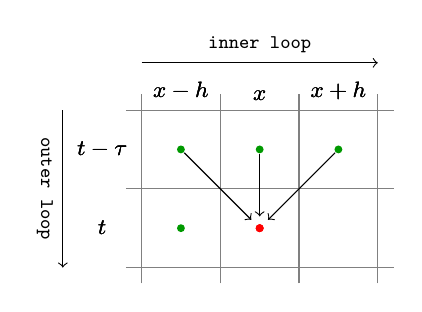
\begin{tikzpicture}
                \draw[->] (0,2.6) -- (3,2.6) node[midway,above] {\scriptsize \texttt{inner loop}};
                \draw[->] (-1,2) -- (-1,0) node[midway,rotate=270,below] {\scriptsize \texttt{outer loop} };
                \draw[step=1,gray] (-0.2,-0.2) grid (3.2,2.2);
                \begin{scope}[yshift=-5mm,xshift=-5mm]
                    \foreach \x/\y in {1/2, 2/2, 3/2, 1/1} {
                            \fill[black!40!green] (\x,\y) circle (0.5mm);
                        }
                    \foreach \x/\y in {1/2, 2/2, 3/2} {
                            \draw[->, shorten >= 1.5mm, shorten <= 0.6mm] (\x,\y) -- (2,1);

                            \fill[red] (2,1) circle (0.5mm);

                            \node at (1,2.5) [above] {\footnotesize $x-h$};
                            \node at (2,2.5) [above] {\footnotesize $x$};
                            \node at (3,2.5) [above] {\footnotesize $x+h$};
                            \node at (0,2) {\footnotesize $t-\tau$};
                            \node at (0,1) {\footnotesize $t$};
                        }
                \end{scope}
            \end{tikzpicture}
        }
        \caption{Evaluation of \texttt{V} at a single-step $x$ (i.e. the inner for-loop) in the FTCS method. All green dots are known, and red is the unknown value being evaluated.}
        \label{fig:Graphftcs}
    \end{figure}
}

\def\figBorderDD
{
    \begin{figure}[H]
        \centering
        {
            \begin{tikzpicture}
                % \draw[step=0.5cm, gray, very thin] (0,0) node[black, above=5mm] {$-L/2$} grid (8,0.5) node[black, above] {$+L/2$};
                \draw[step=0.5cm, gray, very thin] (0,0) grid (3.2,0.5);
                \draw[step=0.5cm, gray, very thin] (4.8,0) grid (8,0.5);
                \draw[|<->|] (-0.5,-0.5) -- (8.5,-0.5);
                \draw[|-|] (1,0.7) -- (1.5,0.7);
                \draw[|->] (4,-0.15) node[below] {$_o$} -- (4.5,-0.15) node[right] {$x$};
                \node at (1.25,0.7) [above] {$h$};
                \node at (-0.5,-0.5) [left] {$-L-h$};
                \node at (8.5,-0.5) [right] {$+L+h$};
                \node at (4,-0.5) [below] {$2L+2$};
                \foreach \x in {3.5,4,4.5} {
                        \foreach \y in {0.25} {
                                \fill[black] (\x, \y) circle (0.5mm);
                            }

                        \draw[step=0.5cm, gray, very thin, red] (7.99,0) grid (8.5,0.5);
                        \draw[step=0.5cm, gray, very thin, red] (-0.5,0) grid (0.01,0.5);
                    }
            \end{tikzpicture}
        }
        \caption{Discretized domain \autoref{fig:DescretizedDomain} with boundaries.}
        \label{fig:BorderDD}
    \end{figure}
}


\def\figHalo
{
    \begin{figure}[H]
        \centering
        {
            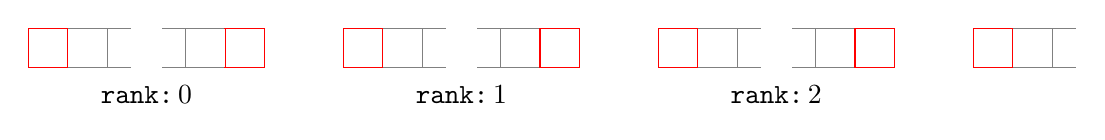
\begin{tikzpicture}
                % \draw[step=0.5cm, gray, very thin] (0,0) node[black, above=5mm] {$-L/2$} grid (8,0.5) node[black, above] {$+L/2$};
                \begin{scope}
                    \pgfmathsetmacro{\yvalb}{-2.5}
                    \pgfmathsetmacro{\yvala}{-2}

                    \foreach \x in {0,4,8,12} {
                            \begin{scope}[xshift=\x cm]
                                \draw[step=0.5cm, red] (-1.5,\yvala) grid (-1,\yvalb);
                                \draw[step=0.5cm, gray, very thin] (-0.99,\yvala) grid (-0.19,\yvalb);
                            \end{scope}
                        }

                    \foreach \x in {0,4,8} {
                            \begin{scope}[xshift=\x cm]
                                \draw[step=0.5cm, red] (0.99,\yvala) grid (1.5,\yvalb);
                                \draw[step=0.5cm, gray, very thin] (0.2,\yvala) grid (0.99,\yvalb);
                            \end{scope}
                        }
                    \foreach \x/\L in {0/0,4/1,8/2} {
                        \begin{scope}[xshift=\x cm]
                            \node at (0,\yvalb-.1) [below] {$\texttt{rank:}\, \L$};
                        \end{scope}
                    }
                \end{scope}
                % \draw[thick,->] (0,0) -- (0,-4) node[midway, fill=white, inner sep=1pt] {Text Label};

            \end{tikzpicture}
        }
        \caption{\texttt{create\_halo()} creates borders at each local discretization which is needed to implement the initial condition and sharing values.}
        \label{fig:Halo}
    \end{figure}
}

\def\figParftcs
{
    \begin{figure}[H]
        \centering
        {
            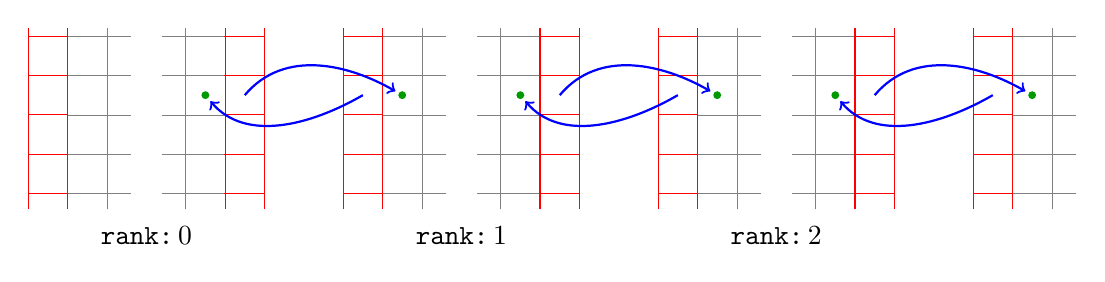
\begin{tikzpicture}
                % \draw[step=0.5cm, gray, very thin] (0,0) node[black, above=5mm] {$-L/2$} grid (8,0.5) node[black, above] {$+L/2$};

                \begin{scope}
                    \pgfmathsetmacro{\yvalb}{-4.2}
                    \pgfmathsetmacro{\yvala}{-1.9}

                    \foreach \x in {0,4,8,12} {
                            \begin{scope}[xshift=\x cm]
                                \draw[step=0.5cm, red] (-1.5,\yvala) grid (-1,\yvalb);
                                \draw[step=0.5cm, gray, very thin] (-0.99,\yvala) grid (-0.19,\yvalb);
                            \end{scope}
                        }

                    \foreach \x in {0,4,8} {
                            \begin{scope}[xshift=\x cm]
                                \draw[step=0.5cm, red] (0.99,\yvala) grid (1.5,\yvalb);
                                \draw[step=0.5cm, gray, very thin] (0.2,\yvala) grid (0.99,\yvalb);
                            \end{scope}
                        }
                    \foreach \x/\L in {0/0,4/1,8/2} {
                            \begin{scope}[xshift=\x cm]
                                \node at (0,\yvalb-.1) [below] {$\texttt{rank:}\, \L$};
                            \end{scope}
                        }

                    \foreach \x in {0,4,8} {
                            \begin{scope}[xshift=\x cm]
                                \draw[->, thick, blue, shorten >= 1mm] (1.25,-2.75) to[out=50, in=150] (3.25,-2.75);
                                \draw[->, thick, blue, shorten >= 1mm] (2.75,-2.75) to[out=-150, in=-50] (0.75,-2.75);
                                \fill[black!40!green] (3.25,-2.75) circle (0.5mm);
                                \fill[black!40!green] (0.75,-2.75) circle (0.5mm);
                            \end{scope}
                        }

                \end{scope}
            \end{tikzpicture}
        }
        \caption{Sharing of bordering values at each time-step. As \texttt{rank:0} doesn't have a left neighbour, it only performs \texttt{Sendrecv()} on the right. The last \texttt{rank} would behave similarly}
        \label{fig:Parftcs}
    \end{figure}
}